\documentclass{article}
\usepackage{amsmath,amssymb}
\usepackage{xcolor}
\usepackage{graphicx}        % for \includegraphics
\graphicspath{{./}{images/}} % adjust or add subfolders here
\usepackage{geometry}
\geometry{a4paper, margin=1in}

\title{derivation of FEM for extended Euler--Bernoulli beam (Quadratic axial + Cubic bending)}
\author{}
\date{}

\begin{document}
	\maketitle
	
	\section*{Step 1: quadratic axial element (mapping from \(x\)-domain to \(\boldsymbol{\xi}\)-domain)}
	
	We define the element over \(x\in[x_1,x_2]\).  To simplify integrals, map to \(\xi\in[-1,1]\):
	\[
	x = \frac{L_e}{2}\,\xi + \frac{x_1+x_2}{2}
	\quad\Longrightarrow\quad
	\frac{d}{dx} = \frac{2}{L_e}\,\frac{d}{d\xi}.
	\]
	Interpolate axial displacement as
	\[
	u(\xi) = N_1(\xi)\,u_1 + N_2(\xi)\,u_m + N_3(\xi)\,u_2,
	\]
	with
	\[
	N_1(\xi)=\tfrac12\,\xi(\xi-1),\quad
	N_2(\xi)=1-\xi^2,\quad
	N_3(\xi)=\tfrac12\,\xi(\xi+1).
	\]
	Compute strain:
	\[
	\varepsilon(\xi)
	= \frac{du}{dx}
	= \frac{2}{L_e}\,\frac{du}{d\xi}
	= \frac{2}{L_e}\,B^{(u)}(\xi)
	\begin{bmatrix}u_1\\u_m\\u_2\end{bmatrix},
	\]
	where
	\[
	B^{(u)}(\xi)
	= \begin{bmatrix}\xi-\tfrac12 & -2\xi & \xi+\tfrac12\end{bmatrix}.
	\]
	Thus the axial stiffness matrix is
	\[
	k_e^{(\mathrm{axial})}
	= EA \int_{-1}^1 (B^{(u)})^T B^{(u)}\,\frac{L_e}{2}\,d\xi
	= \frac{2EA}{L_e}
	\begin{bmatrix}
		\tfrac76 & -\tfrac43 & \tfrac16\\
		-\tfrac43 & \tfrac83 & -\tfrac43\\
		\tfrac16 & -\tfrac43 & \tfrac76
	\end{bmatrix}.
	\]
	
	\section*{Step 2: Cubic bending element derivation}
	
	With Hermite cubic shape functions \(N_1^{(w)},\dots,N_4^{(w)}\):
	\[
	w(\xi)
	= N_1^{(w)}\,w_1 + N_2^{(w)}\,\theta_1
	+ N_3^{(w)}\,w_2 + N_4^{(w)}\,\theta_2,
	\]
	and curvature
	\[
	\kappa = -\frac{d^2w}{dx^2}
	= -\Bigl(\tfrac{2}{L_e}\Bigr)^2 \frac{d^2w}{d\xi^2}.
	\]
	The bending stiffness becomes
	\[
	k_e^{(\mathrm{bending})}
	= \int_{-1}^1 EI
	\Bigl(\tfrac{d^2N}{dx^2}\Bigr)^T
	\Bigl(\tfrac{d^2N}{dx^2}\Bigr)\,\frac{L_e}{2}\,d\xi
	= \frac{EI}{L_e^3}
	\begin{bmatrix}
		12     & 6L_e   & -12   & 6L_e \\
		6L_e   & 4L_e^2 & -6L_e & 2L_e^2 \\
		-12    & -6L_e  & 12    & -6L_e \\
		6L_e   & 2L_e^2 & -6L_e & 4L_e^2
	\end{bmatrix}.
	\]
	
	\section*{Step 3: Merge axial and bending}
	
	Using DOFs \(\{u_1,w_1,\theta_1,u_m,u_2,w_2,\theta_2\}\),
	\[
	k_e
	= \begin{bmatrix}
		k_{3\times3}^{(\mathrm{axial})} & \mathbf{0} \\
		\mathbf{0} & k_{4\times4}^{(\mathrm{bending})}
	\end{bmatrix}.
	\]
	
	\section*{Step 4: Apply boundary conditions}
	
	For a fixed–fixed element:
	\[
	u_1=w_1=\theta_1=0,\quad
	u_2=w_2=\theta_2=0.
	\]
	Remove those rows and columns from the global \(K\) and \(F\).
	
	\section*{Step 5: Solve for displacement}
	
	After reduction:
	\[
	K_{\mathrm{red}}\,U = F_{\mathrm{red}}
	\quad\Longrightarrow\quad
	U = K^{-1}F.
	\]
	
	\section*{llustration of the beam element}
	\begin{figure}[ht]
		\centering
		% Put your image file (e.g. Quadratic_Axial.png) in the same folder or in ./images/
		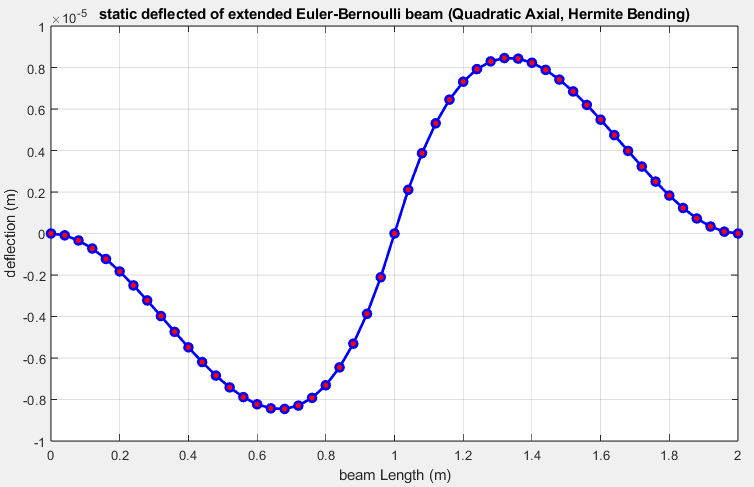
\includegraphics[width=0.8\textwidth]{Quadratic_Axial.png}
		\caption{Schematic of the deflection extended Euler--Bernoulli beam element by applying moment at the middle of the beam}
		\label{fig:beam-element}
	\end{figure}
	
\end{document}
